\documentclass{dcthesis}

%This version of the thesis template has been updated for the February 2017 thesis guidelines provided by the School of Graduate and Advanced Studies by David Freund and Daryl DeFord.

%  Some good options are draft and singlespacing, for drafts, and *final*,
%for the final cut, and noheadings, for a printout without headings.  
%You can also use the copyright option to add a copyright.  Note:
%final will enforce a bunch of different options, like oneside, 12pt
%and doublespacing, as well as make the margins correct.   Draft, has
%larger margins and is appropriate for twosided printing.   


%%%%%%%%%%%%%%%%%%%%%%%%%%%
%%%%    IMPORTANT     %%%%%
%%%%%%%%%%%%%%%%%%%%%%%%%%%
%
%  Because dvips doesn't know/care about the page size of the dvi file
%  its working on, and because its so important that the margins of
%  your thesis are correct you have to make sure that you are using
%  the command dvi -t letter *thesisnamehere*
%
%  If you are using a terminal this is straightforward, but if you are
%  using a tex editing program it make take a little bit of searching
%  before you figure out how to make this work. 
%  
%  Alternatively, you might consider compiling using pdflatex, which
%  compiles straight to a PDF and doesn't have this problem.  

%%%%%%%%%%%%%%%%%%%%%%%%%%%%%%%%%%%%%%%%%%%%%%%%%%
% Some Defaults
%%%%%%%%%%%%%%%%%%%%%%%%%%%%%%%%%%%%%%%%%%%%%%%%%%
\committee[F. Jon Kull, Ph.D.]{}{}{}{}
\school{Dartmouth College}{Hanover, New Hampshire}
\degree{Doctor of Philosophy}
\field{Mathematics}

%%%%%%%%%%%%%%%%%%%%%%%%%%%%%%%%%%%%%%%%%%%%%%%%%%
% Additional Packages (add as desired)
%%%%%%%%%%%%%%%%%%%%%%%%%%%%%%%%%%%%%%%%%%%%%%%%%%
\usepackage{amsmath,amssymb,amsthm}
\usepackage{natbib}
\usepackage{times}
\usepackage{latexsym}
\usepackage{titlesec}
\usepackage{color,soul}
\usepackage{hyperref}
\renewcommand{\UrlFont}{\ttfamily\small}
\usepackage{graphicx}
\graphicspath{{./images/}}
%\usepackage[parfill]{parskip}
\usepackage{booktabs}
\usepackage{array}
\usepackage{microtype}
\usepackage{caption}
\usepackage{tablefootnote}
\usepackage{float}

\newcommand{\comment}[1]{}

%\usepackage{mkindex} %Uncomment if you would like to have an index. Compiling with an index takes more work than compiling without one. You will have to look up how to use the index package.

%%%%%%%%%%%%%%%%%%%%%%%%%%%%%%%%%%%%%%%%%%%%%%%%%%
%Formatting
%%%%%%%%%%%%%%%%%%%%%%%%%%%%%%%%%%%%%%%%%%%%%%%%%%
%  Change or add to as desired. 
%  These two commands make the first enumerations look like (a)
%  And the second level like (i).  
\renewcommand{\labelenumi}{(\alph{enumi})}
\renewcommand{\labelenumii}{(\roman{enumii})}
%  These commands make the section headings Boldface and not all
%  caps. It also removes the chapter numbers  
\renewcommand{\chaptermark}[1]{\markboth{{\sc #1}}{{\sc #1}}}
\renewcommand{\sectionmark}[1]{\markright{{\sc \thesection\ #1}}}
%  These commands have lowercase headings with chapter numbers. 
%\renewcommand{\chaptermark}[1]{markboth{#1}{}}
%\renewcommand{\sectionmark}[1]{\markright{\thesection\ #1}} 
		
%%%%%%%%%%%%%%%%%%%%%%%%%%%%%%%%%%%%%%%%%%%%%%%%%%
% Theorem Declarations
%%%%%%%%%%%%%%%%%%%%%%%%%%%%%%%%%%%%%%%%%%%%%%%%%%
% A basic set of theorem declarations.  Add or remove as desired. 
\newtheorem{prop}{Proposition}[chapter]
\newtheorem{theorem}[prop]{Theorem}
\newtheorem{lemma}[prop]{Lemma}
\newtheorem{corr}[prop]{Corollary}
\theoremstyle{definition}
\newtheorem{definition}[prop]{Definition}
\theoremstyle{remark}
\newtheorem{remark}[prop]{Remark}
\newtheorem{example}[prop]{Example}
\newtheorem*{claim}{Claim}

%%%%%%%%%%%%%%%%%%%%%%%%%%%%%%%%%%%%%%%%%%%%%%%%%%
%Indicies
%%%%%%%%%%%%%%%%%%%%%%%%%%%%%%%%%%%%%%%%%%%%%%%%%%
%This is for an index.  More work is neede for a notation index
%\makeindex

%%%%%%%%%%%%%%%%%%%%%%%%%%%%%%%%%%%%%%%%%%%%%%%%%%
% Macros
%%%%%%%%%%%%%%%%%%%%%%%%%%%%%%%%%%%%%%%%%%%%%%%%%%
% Add your math macros here

%%%%%%%%%%%%%%%%%%%%%%%%%%%%%%%%%%%%%%%%%%%%%%%%%%
% Title Page Information
%%%%%%%%%%%%%%%%%%%%%%%%%%%%%%%%%%%%%%%%%%%%%%%%%%
%  Your personal info goes here!
\title{BigGreen at SemEval-2021 Task 1: \\Lexical Complexity Prediction with Assembly Models}
\author{Aadil Islam}
\date{May 2021}
\field{Computer Science}
\degree{Bachelor of Arts}
%As an optional arguement to \committee you can specify the dean of graduate studies.
\committee{LGF}{The Mustache}{The Big Cheese}{Totally Real Subfield}

\begin{document}

%%%%%%%%%%%%%%%%%%%%%%%%%%%%%%%%%%%%%%%%%%%%%%%%%%
%Front end of thesis
%%%%%%%%%%%%%%%%%%%%%%%%%%%%%%%%%%%%%%%%%%%%%%%%%%
\frontmatter

\newgeometry{left=1.5in,top=1in,bottom=1in,right=1in}
\maketitle
\restoregeometry

%%%%%%%%%%%%%%%%%%%%%%%%%%%%%%%%%%%%%%%%%%%%%%%%%%
%Abstract
%%%%%%%%%%%%%%%%%%%%%%%%%%%%%%%%%%%%%%%%%%%%%%%%%%
%NOTE:  Must be less than 350 words.  
\chapter*{Abstract}
%This is so the abstract appears in the ToC
\addcontentsline{toc}{section}{Abstract}
This paper describes systems submitted by team BigGreen to LCP 2021. We assemble a feature engineering-based model with a deep neural network model founded on BERT. The latter model contextualizes a target expression, given its sentence. While BERT is a strong model overall, the feature engineering-based model helps in extreme cases, eg. separating instances of easy and neutral difficulty. Our handcrafted features comprise a breadth of lexical, semantic, syntactic, and novel phonological measures. Additionally, visualizations of BERT attention maps offer insight into potential features that Transformers models may learn when fine-tuned for lexical complexity prediction. Our ensembled predictions score reasonably well for the single word subtask, and we demonstrate how they can be harnessed to perform well on the multi word expression subtask too.

\chapter*{Acknowledgments}
\addcontentsline{toc}{section}{Acknowledgments}

I was fortunate to have been mentored by graduate student Weicheng Ma and Professor Soroush Vosoughi. I owe everything to their invaluable guidance and encouragement that inspired me this past year, which has motivated me to pursue future academic research. Finally, I thank the College's Research Information, Technology and Consulting (RITC) department for providing me computational resources necessary to complete my research.

%%%%%%%%%%%%%%%%%%%%%%%%%%%%%%%%%%%%%%%%%%%%%%%%%%
%Table of Contents
%%%%%%%%%%%%%%%%%%%%%%%%%%%%%%%%%%%%%%%%%%%%%%%%%%
\tableofcontents

%Add a list of tables
%\listoftables

%Add a list of figures
%\listoffigures

%%%%%%%%%%%%%%%%%%%%%%%%%%%%%%%%%%%%%%%%%%%%%%%%%%
%Main Portion of Thesis
%%%%%%%%%%%%%%%%%%%%%%%%%%%%%%%%%%%%%%%%%%%%%%%%%%
\mainmatter

%%%%%%%%%%%%%%%%%%%%%%%%%
%%  YOUR THESIS HERE!  %%
%%%%%%%%%%%%%%%%%%%%%%%%%

\chapter{Introduction}

Lexical simplification (LS) is the task of replacing difficult words in a text with simpler alternatives. It is applicable to reading comprehension, where early studies have shown infrequent words to lead to more time a reader spends fixated on it, and that ambiguity in a word's meaning further adds to comprehension time \citep{raynerd86}. \citet{devlin} demonstrate that a combined approach studying both the \textit{syntactic} structure of a context (where certain compositions may be more difficult to understand than others) and the \textit{lexical} characteristics of each word (certain words are more frequent in language than other) can be used to simplify challenging texts for individuals suffering from aphasia. Complex word identification (CWI) is believed to be a fundamental step in the automation of lexical simplification \citep{shardlow2014open}. 
Early techniques for conducting CWI, however, lack in robustness at the word level, from initially simplifying all words in given a sentence to then observe incurred change in meaning \citep{devlintait}, to applying simple thresholds on discriminative features like word frequency \citep{10.1007/11573067_19}.

The recent CWI shared task at SemEval-2016 \citep{paetzoldspecia:2016:SemEval1} studied the annotations of 400 non-native speakers on English target words, labeled as either simple or complex. The SemEval-2018 CWI shared task \citep{stajner-EtAl:2018:BEA} extended their study to data across four languages, while also introducing a probabilistic component to the binary classification task. This year's Lexical Complexity Prediction (LCP) shared task \citep{shardlow2020complex} forgoes the treatment of word difficulty as a binary classification task \citep{paetzoldspecia:2016:SemEval1, stajner-EtAl:2018:BEA} and instead measures degree of difficulty on a continuous scale. This choice is intriguing as it mitigates a dilemma with previous approaches of having to treat words close to a decision boundary (suppose a threshold deems a word's difficulty) identically to those that are far away, ie. extremely easy or difficult.

Teams are asked to submit predictions on unlabeled test sets for two subtasks: predicting on single word and multi word expressions (MWEs), respectively. The Pearson correlation coefficient is used to evaluate how closely submitted predictions associate with ground truth labels. For each subtask, \texttt{BigGreen} presents a machine learning-based approach that fuses the predictions of a feature engineering-based regressor with those of a feature learning-based deep neural network model founded on BERT \citep{DBLP:journals/corr/abs-1810-04805}. Our code is made fully available on GitHub.\footnote{\url{https://github.com/Aadil101/BigGreen-at-LCP-2021}}

In Sections 2 and 3 of this paper, we overview related work that inspires our experiments and describe the data used to train \texttt{BigGreen}'s models. For the feature engineering-based model, Section 4 explains six categories of linguistic features experimented with, in addition to feature selection techniques; for the feature learning-based model, we describe its training procedure here. Sections 5 and 6 show how our approaches performed in competition, as well as analysis on worked and what did not.

\chapter{Related Work}

Previous studies have looked at estimating the readability of a given text, though at the sentence-level rather than word-level. \citet{10.2307/40011226} regresses the number of polysyllabic words in a given lesson against the mean score for students quizzed on information pertaining to the lesson, yielding the SMOG Readability Formula. \citet{10.2307/1473169} offer a list of 768 (later updated to 3,000) words familiar to grade-school students in reading, which they find correlates with the relative difficulty of a given passage. An issue with traditional readability metrics seems to be the loss of generality at the word-level.

\citet{shardlow2013comparison} tries a brute force approach where a simplification algorithm is applied to each word of a given text, deeming a world complex if simplified. However, this suffers from the assumption that a non-complex word does not require further simplification. Also attempted is the assignment of familiarity scores to each word, where a threshold that determining a word's complexity is tuned \citep{shardlow2013comparison}. We avoid thresholding in our study because we find it unnecessary, since raw familiarity scores can be used as features in regression-based tasks. 

Results for the SemEval-2016 task \citep{zampieriEtAl:2017:NLPTEA} suggest that vote ensembling predictions of one's best performing models to be an effective strategy, while several top-performing models appear to use linguistic information beyond just word frequency \citep{paetzoldspecia2016sv000gg, ronzanoetal2016taln, mukherjeeetal2016ju}; namely, they include lexical, semantic, syntactic, and psycholinguistic features. These findings inspire our use of ensemble techniques, as well us our consideration of phonological features as a new area of research. Results from SemEval-2018 show feature engineering-based models outperforming deep learning-based counterparts, despite the latter having generally better performances since SemEval-2016.

\chapter{Data Collection}

\section{CompLex Dataset}

\begin{table}
  \centering
  \begin{tabular}{l|l|r|r|r}
    \hline
    \centering
    \textbf{Corpus} & \textbf{Subtask} & \textbf{Train} &  \textbf{Trial} &  \textbf{Test} \\
    \hline
    Bible & Single Word &   2574 &    143 &   283 \\
            & Multi Word &    505 &     29 &    66 \\
    Biomed & Single Word &   2576 &    135 &   289 \\
            & Multi Word &    514 &     33 &    53 \\
    Europarl & Single Word &   2512 &    143 &   345 \\
            & Multi Word &    498 &     37 &    65 \\
    \hline
    \textbf{Total} & Single Word & 7662 & 421 & 917 \\
          & Multi Word &    1517 &     99 &    184 \\
    \hline
  \end{tabular}
  \caption{\label{tab:datasets} LCP train, trial, and test sets.}
\end{table}

\citet{shardlow2020complex} present CompLex, a novel dataset in which each target expression (single word or MWE) is assigned a continuous label denoting its lexical complexity. Each label falls in range 0-1, a (normalized) average score given by employed crowd workers who report a given expression's difficulty on a 5-point Likert scale. Note that all crowd workers originate from English speaking countries (UK, USA, and Australia). We define a sample's \textit{class} as the bin to which its complexity label belongs (bins corresponding to Likert points). Target expressions in CompLex have 0.395 average complexity and 0.115 standard deviation, reflecting an imbalance in favor of class 2 and 3 samples.

Each target expression is accompanied by the sentence it was extracted from, where certain target words appear multiple times in the dataset (in different contexts). A target expression is drawn from one of three sources (Bible, Biomed, and Europarl) in an effort to motivate study of domain-specific linguistic features. As noted by \citet{shardlow2020complex}, Biomed samples appear to be on average 1.7 and 2.2 percent higher in lexical complexity than Bible and Europarl samples, respectively. This we believe may reflect the elevated diction exhibited in biomedical research and academic writing in general, a style of language that differs from typical colloquial dialogue used in biblical scripture or parliamentary debates. Although an annotator's predisposition to theology, academia, and/or politics may affect their labeling of samples in CompLex, this component is sadly beyond the scope of this study. A summary of train, trial,\footnote{In our study we avoid the trial set as we find it to be less representative of the training data, opting instead for training set cross-validation, stratified by corpus and complexity label.} and test set samples is given in Table \ref{tab:datasets}.

\section{External Datasets}

In this study, we use four additional corpora to extract term frequency-based features for training our feature engineering-based model:

\begin{itemize}
  \item \textbf{English Gigaword Fifth Edition} (Gigaword): this comprises articles from seven prominent international English newswires, acquired by the Linguistic Data Consortium (LDC) \citep{gigaword}.
  \item \textbf{Google Books Ngrams, version 2} (GBND): this is used to count occurences of phrases across a corpus of books, accessed via the PhraseFinder API \citep{phrasefinder}.
  \item \textbf{British National Corpus, version 3} (BNC): this is a 100 million word collection of British written and spoken English \citep{BNC}.
  \item \textbf{SUBTLEXus}: this consists of American English subtitles totaling 51 million in words, whose creators offer a multitude of word frequency lists for \citep{Brysbaert2009MovingBK}.
\end{itemize}

\chapter{Data Exploration}

\begin{table}[]
    \centering
    \begin{tabular}{l|c|c|c|c}
    \hline
     & \textbf{All} & \textbf{Handcrafted} & \textbf{GloVe word+context} & \textbf{InferSent} \\
    \hline
    \textbf{All} & 0.1399 & 0.0964 & 0.0749 & 0.1585 \\
    \textbf{Bible} & 0.1133 & 0.0986 & 0.0884 & - \\
    \textbf{Biomed} & - & 0.1094 & 0.0852 & 0.2060 \\
    \textbf{Europarl} & - & 0.0762 & 0.0698 & - \\
    \hline
    \end{tabular}
    \caption{\label{tab:baseline_systems} The results of linear regression with different baseline feature subsets. All results are reported in terms of mean absolute error (MAE). Note that \textbf{GloVe word+context} denotes the concatenation of 300-dim GloVe word and 300-dim GloVe context embeddings. A hyphen `-' denotes an extremely high MAE.}
\end{table}

\begin{table}[]
    \centering
    \begin{tabular}{ccp{0.6\linewidth}cl}
    \hline
    \multicolumn{1}{c}{\textbf{ID}} & \multicolumn{1}{c}{\textbf{Corpus}} & \multicolumn{1}{c}{\textbf{Context}} & \textbf{Complexity} &  \\
    \hline
    1 & Bible & Now God made Daniel to find kindness and compassion in the sight of the prince of the \textbf{eunuchs}. & 0.632 &  \\
    2 & Bible & he sent Hadoram his son to king David, to Greet him, and to bless him, because he had fought against Hadadezer and struck him; (for Hadadezer had wars with \textbf{Tou};) and he had with him all kinds of vessels of gold and silver and brass. & 0.825 &  \\
    3 & Biomed & During budding morphogenesis, intersecting signaling networks from the epithelium and mesenchyme govern transcriptional, adhesive, polarity, and \textbf{motility} programs in these select groups of cells. & 0.714 &  \\
    4 & Biomed & Future fine mapping experiments can be designed to randomize the influences of any contaminating donor \textbf{alleles} and environmental differences, as well as test for maternal genotype effects. & 0.625 &  \\
    5 & Biomed & In the development of the mammalian retina, a diverse \textbf{range} of cell types is generated from a pool of multipotent retinal progenitor cells. & 0.050 &  \\
    6 & Biomed & In the mouse model of \textbf{RA}, small genetic contributions are also often observed. & 0.813 &  \\
    7 & Biomed & As in our tet-off \textbf{APP} mice, SantaCruz et al. found that tau neurofibrillary tangles, like amyloid plaques, are not cleared efficiently following transgene suppression. & 0.692 &  \\
    8 & Biomed & These mice were mated with a strain carrying \textbf{Cre} recombinase under the control of the human Keratin 14 (K14) promoter, which is active in basal cells of epidermis and other stratified epithelia. & 0.783 &  \\
    9 & Europarl & Once there is a statute based on equality, Madam President, the rules for travel and \textbf{subsistence} expenses can also be changed. & 0.486 &  \\
    10 & Europarl & Mobilisation of the European \textbf{Globalisation} Adjustment Fund: Ireland - SR Technics ( & 0.611 & \\
    \hline
    \end{tabular}
    \caption{\label{tab:samples} Ten of the top-50 samples predicted with large error margins (MAE) by multiple variant baseline systems. Each sample's target word is bolded.}
\end{table}

\begin{figure}
    \centering
    \begin{minipage}[b]{0.45\textwidth}
        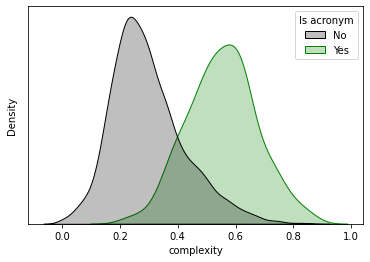
\includegraphics[width=\textwidth]{is_acronym.png}
        \caption{\label{fig:is_acronym} Probability density functions for acronym vs. non-acronym target words in single word training set.}
    \end{minipage}
    \hfill
    \begin{minipage}[b]{0.45\textwidth}
        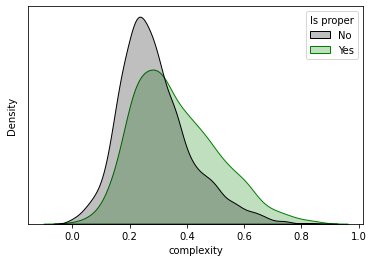
\includegraphics[width=\textwidth]{is_proper.png}
        \caption{\label{fig:is_proper} Probability density functions for proper vs. improper noun/adjective target words in single word training set.}
    \end{minipage}
\end{figure}

\section{Assessing Baseline Systems}

We focus initially on the single word subtask by experimenting with a baseline system inspired by that of the authors of CompLex \citep{shardlow2020complex}. Our goal in using this modified baseline system is to identify successful predictors, and to understand the shortcomings of said feature set, guiding the construction of BigGreen's own systems. The baseline system comprises a series of handcrafted features, GloVe word embeddings \citep{pennington2014glove}, GloVe context embeddings (kindly see Section \ref{paper:semantic_features} for more on this) and InferSent sentence embeddings \citep{conneau-EtAl:2017:EMNLP2017}. The handcrafted features include (1) target word frequency, courtesy of the Wordfreq library \citep{robyn_speer_2018_1443582}, (2) word length, and (3) syllable count, courtesy of the Syllables library.\footnote{\url{https://github.com/prosegrinder/python-syllables}}. 

As shown in Table \ref{tab:baseline_systems}, performances of variant baseline systems (a \textit{variant} being a fitting over some subset of the aforementioned features) show promise in the use of all handcrafted lexical features, and successes with certain semantic features (eg. GloVe word embeddings, but not InferSent sentence embeddings). 

\section{Examining Challenging Samples}

We manually assess training set samples that multiple variant baseline systems struggled with, samples that are perhaps naturally difficult to predict on; Table \ref{tab:samples} shows some of these. Observe that samples 6 and 7 bear target words that are acronyms, terms like \lq{RA}\rq and \lq{APP}\rq{} whose meanings are perhaps assumed to be common knowledge to academic audiences. Samples 2, 8, and 10 have target words that are proper nouns and adjectives, usually referring to domain-specific entities that cannot necessarily be learned from context clues (eg. samples 2 and 8 seem to expect the reader to know what \lq{Tou}\rq{} and \lq{Cre}\rq{} are). Figures \ref{fig:is_acronym} and \ref{fig:is_proper} illustrate the effects of acronymity and propriety to perceived target word complexity.

Finally, we notice that target words used rarely in language (eg. Samples 1, 3, 4, and 9) need to be better considered by future systems. Moreover, we hypothesize that N-grams comprising a target word affect its perceived complexity; the target word in sample 5 is often used in the phrase \lq{\textbf{range} of,}\rq{} whereas the target word in sample 4 rarely ever arises in a niche noun phrase like \lq{contaminating donor \textbf{alleles}.}\rq{} 

\section{Character Transition Probabilities}

\begin{table}
  \centering
  \begin{tabular}{c|ccc|cc}
    \hline
    \centering
    & \multicolumn{3}{c|}{\textbf{Character Transition Probability}} &  &  \\
    \textbf{Char. Transition} & \textbf{Gigaword} & \textbf{Class 1} & \textbf{Class 4, 5} & \textbf{T-Statistic} & \textbf{P-Value}  \\
    \hline
    $i \rightarrow d$ & 0.0597 & 0.0331 &  0.0588 &    -7.3532 &  4.5127e-10 \\
    $o \rightarrow s$ & 0.0402 & 0.0200 &  0.0976 &    -4.4796 &  2.7255e-05 \\
    $o \rightarrow r$ & 0.1568 & 0.1233 &  0.1463 &    -2.1475 &  1.6440e-02 \\
    $y \rightarrow c$ & 0.0129 & 0.0500 &  0.3333 &    -1.8898 &  5.8693e-02 \\
    $p \rightarrow h$ & 0.0206 & 0.0156 &  0.4500 &    -1.5407 &  6.8241e-02 \\
    $o \rightarrow n$ & 0.2079 & 0.2700 &  0.1707 &    -1.4155 &  7.8776e-02 \\
    $i \rightarrow t$ & 0.1084 & 0.0783 &  0.2353 &    -1.4036 &  8.1026e-02 \\
    $e \rightarrow s$ & 0.1255 & 0.2019 &  0.2143 &    -1.2893 &  9.8986e-02 \\
    \hline
  \end{tabular}
  \caption{\label{tab:top_char_transitions} Character transitions that are more frequent in higher complexity target words (at 10\% significance level). Note that no $y \rightarrow c$ transitions occur across class 3 samples.}
\end{table}

\begin{figure}
  \centering
  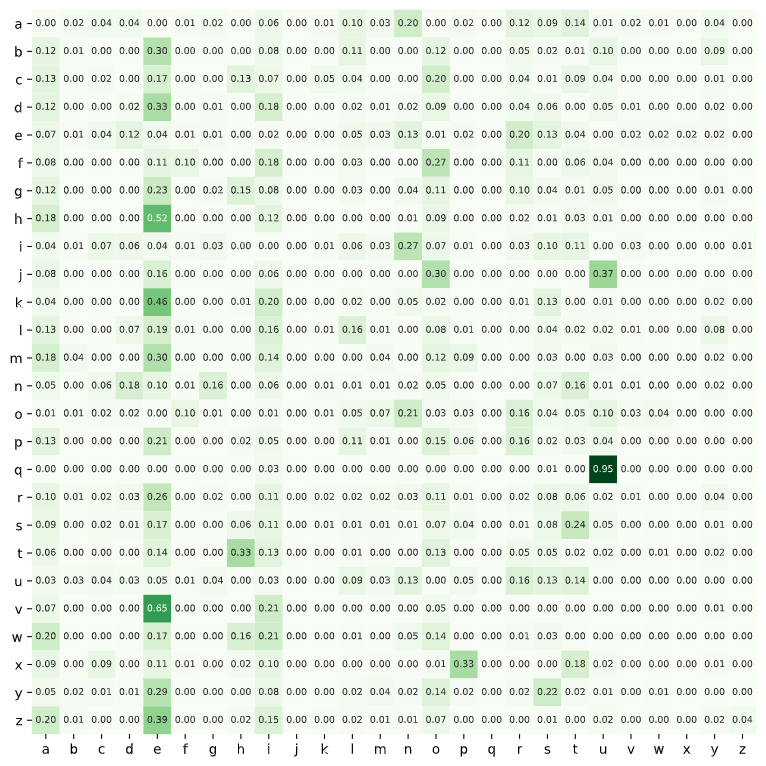
\includegraphics[scale=0.55]{character_transition_probabilities.png}
  \captionsetup{justification=centering}
  \caption{\label{fig:character_transition_probabilities} Lowercase ASCII transition probabilities, estimated using Gigaword.}
\end{figure}

While prior top-performing approaches harness a variety of  linguistic information across lexical, semantic, syntactic, and psycholinguistic features \citep{paetzoldspecia2016sv000gg, ronzanoetal2016taln, mukherjeeetal2016ju}, there appears to be a lack of consideration of phonological features. \citet{doi10108000437956195011659381} suggests that the relative frequencies of phonemes can be used to potentially identify important phonemes to tutor foreign language students with who exhibit numerous phonemic difficulties. While we assume that each crowd annotator of CompLex understand at least one dialect of English, we also assume for convenience that they share similar literacy levels and general familiarity with the English language. We hypothesize that because certain English phonemes (ie. soundable segments or character n-grams) are evidently more common in usage than others \citep{doi10108000437956195011659381}, a target word's complexity could be impacted by an annotator's familiarity with its constituent phonemes.

For a given target word $w$, consider the transition probability from character $w[i]$ to the character $w[i+1]$, that is, the expected probability of the $(i+1)$th character succeeding the $i$th character in language; we call this a \textit{character} transition probability. To understand whether this may be a useful feature for our task, for each target word $w$ of class $c$, we define the random variable ${}_xT_y \in \mathbb{N}$ as the number of occurences of character transition $x \rightarrow y$ in the target word, where $x, y \in \{\text{ASCII character set}\}$. For each possible transition $x \rightarrow y$, we ask whether the distribution of ${}_xT_y$ over class 1 samples (ie. very easy target words) is different from that over class 4, 5 samples (ie. difficult target words).\footnote{Here, we combine classes 4 and 5 because so few samples exist in each individual class.} Let $\mu_1$ and $\mu_{4,5}$ be the average number of occurences of the given transition $x \rightarrow y$ over  class 1 and class 4, 5 target words, respectively. We conduct an unpaired lower-tailed t-test using the null hypothesis that $H_0\text{: } \mu_1 = \mu_{4,5}$, and the alternative hypothesis that $H_a\text{: } \mu_1 < \mu_{4,5}$. Table \ref{tab:top_char_transitions} presents only the character transitions that yield statistically significant p-values at the 10\% confidence level, implying that these character transitions are slightly more common in higher complexity target words than in lower complexity target words. Note that we also conducted t-tests with instead the alternative hypothesis $H_a\text{: } \mu_1 > \mu_{4,5}$, finding that \textit{no} character transition yields a statistically significant p-value at the 10\% confidence level! 

Perhaps we can intuit some of the character transitions in Table \ref{tab:top_char_transitions}. Notice that character transition probabilities estimated over target word classes lie roughly in the same ballpark as that estimated over the Gigaword corpus; deviation from the Gigaword estimates is somewhat expected considering the relatively small size of the CompLex corpus. Seven of the eight character transitions shown bear higher transition probabilities over class 4, 5 samples compared to over class 1 samples (all except $o \rightarrow n$), perhaps suggesting that target word complexity is correlated with changes in the transition probabilities for particular characters. Based on Figure \ref{fig:character_transition_probabilities}, observe that $y$ often transitions to an $e$, $s$, $o$, etc. whereas rather rarely does it transition to $c$; yet, we find class 4, 5 samples tending to towards this rarity nonetheless, often showing up in scientific words with root `cycl' such as `cycle,' `cyclone,' and `doxycycline.' We observe even more instances of this apparent tendency towards rarer transitions, namely $i \rightarrow d$, $o \rightarrow s$, and $p \rightarrow h$. This subtle pattern suggests that the transition probabilities between characters (and possibly even phonemes) in a target word could serve as a discriminative feature for predicting lexical complexity.

\chapter{BigGreen Systems \& Approaches}

In this section, we overview information fed to the feature engineering-based system, as well as training techniques for the feature learning-based model. We also describe methods for ensembling their predictions for each subtask. Note that the fitted models for the single word subtask are then harnessed for the MWE subtask.

\section{Feature Engineering-based System}

\subsection{Feature Extraction}

We aim to capture a breadth of information pertaining to the target word and its context. The majority of features appear to follow heavily right-skewed distributions, which we attribute to Zipf's law manifesting over our plethora of word frequency-based measures. This prompts us to consider both logged and unlogged versions of features. For the MWE subtask, features are extracted independently for the head and tail words, with they and their \textit{sums} being included in the final feature set.

\subsubsection{Lexical Features}

These features capture lexical information pertaining to the target word:

\begin{itemize}
  \item \textbf{Word length}: length of the target word.
  \item \textbf{Number of syllables}: number of syllables in the target word, via the Syllables library.
  \item \textbf{Is acronym}: whether the target word is a sequence of capital letters.
\end{itemize}
  
\subsubsection{Semantic Features}

\label{paper:semantic_features} These features capture the target word's meaning:

\begin{itemize}
  \item \textbf{WordNet features}: the number of hyponyms and hypernyms associated with the target word in WordNet \citep{Fellbaum:2005}.
  \item \textbf{GloVe word embeddings}: we extract 300-dimension embeddings trained on Wikipedia-2014 and Gigaword \citep{pennington2014glove} for each (lowercased) target word. 
  \item \textbf{ELMo word embeddings}: we extract 1024-dimension embeddings trained on the One Billion Word Benchmark corpus \citep{Peters:2018} for each target word. Observe that these are \textit{contextualized} embeddings, unlike our GloVe word embeddings. 
  \item \textbf{GloVe context embeddings}: we obtain the average 300-dimension GloVe word embedding across all words in the given sentence.
  \item \textbf{InferSent context embeddings}: we obtain 4096-dimension InferSent embeddings \citep{conneau-EtAl:2017:EMNLP2017} for each sentence.
\end{itemize}

\subsubsection{Phonetic Features}

These features compute the likelihood that consecutive soundable segments in the target word would arise in English language. We estimate ground truth transition probabilities between any two units (phonemes or characters) using Gigaword:

\begin{itemize}
  \item \textbf{Phoneme transition probability}: we consider the min/maximum/mean/standard deviation over the set of transition probabilities for the target word's phoneme bigrams. 
  \item \textbf{Character transition probability}: analogous to that above, over \textit{character} bigrams.
\end{itemize}

\subsubsection{Word Frequency \& N-gram Features}

These features are expressly included due to their expected importance, \citep{zampieriEtAl:2017:NLPTEA}. Gigaword is the main corpus from which we extract word frequency measures (for both lemmatized and unlemmatized target words), the summed frequency of a target word's byte pair encodings (BPEs), and summed frequencies of bigrams and trigrams containing the target word. We complement these features with IDF-based analogues. Finally, we use the GBND, BNC, and SUBTLEXus corpora to extract secondary word frequency, bigram, and trigram measures. 

\subsubsection{Syntactic Features}

These are features that assess the syntactic structure of the target word's context. We construct the constituency parse tree for each sentence using a Stanford CoreNLP pipeline \citep{manning-EtAl:2014:P14-5}.

\begin{itemize}
  \item \textbf{Part of speech (POS)}: predicted via NLTK's \texttt{pos\_tag} function \citep{Loper02nltk:the}.
  \item \textbf{Depth of parse tree}: the parse tree's height.
  \item \textbf{Depth of target word}: distance between the target word and parse tree's root node.
  \item \textbf{Number of words at target depth}: number of words at the same depth in the parse tree as the target word.
  \item \textbf{Is proper}: whether target word is a proper noun/adjective, detected via capitalization.
\end{itemize}

\subsubsection{Readability Metrics}

These comprise a variety of tests applied on the target word's context, using low-level traits such as total word count and total syllable count. Interestingly, certain readability metrics count the difficult words in a given sentence by assuming rules for what makes a given word \textit{complex} (eg. the Dale-Chall readability formula \citep{10.2307/1473169} checks a given word against a predetermined list of 3,000 familiar words). This inspires us to try multiple readabililty measures via the Textstat library,\footnote{\url{https://github.com/shivam5992/textstat}} including Flesch-Kincaid grade level, Gunning Fog index, and SMOG index.

\subsection{Feature Selection}

For the single word subtask, we select features using a combination of filter and wrapper methods. Our intention is to leverage successful techniques in the MWE subtask as well, where we extract head and tail-specific features.

\subsubsection{Filter Methods}

\begin{figure}
  \centering
  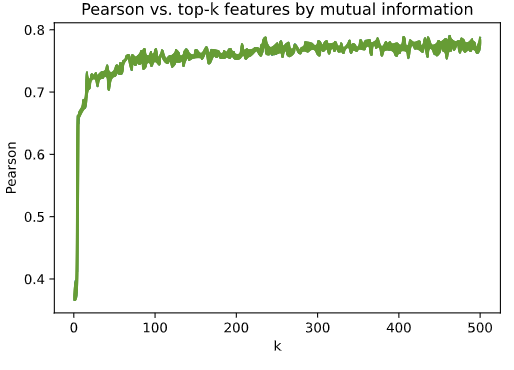
\includegraphics[scale=0.75]{mi.png}
  \caption{\label{fig:mi} Performances of LR fitted (with 5-fold cross-validation) on top-k features by mutual information.}
\end{figure}

\begin{itemize}
  \item \textbf{Variance}: Features are screened by variance of their distributions, with those lower than 0.01 deemed quasi-constant and removed.
  \item \textbf{Mutual Information}: Features are ranked by mutual dependence with lexical complexity, and only the top-$k$ features are selected. We tune $k$ by fitting linear regression models on the top-$k$ features. Figure \ref{fig:mi} shows diminishing improvement in Pearson correlation beyond $k=300$.
  \item \textbf{Variance Inflation Factor (VIF)}: This is computed for each feature to measure contributed multicollinearity. Note that we omit this particular filter method for our submitted model, in order to optimize our model's Pearson correlation coefficient.
\end{itemize}

\subsubsection{Wrapper Methods}

\begin{itemize}
  \item \textbf{Forward Feature Selection (FFS)}: Beginning with an empty feature set, each subsequent iteration appends a feature to the existing feature set offering the best Pearson. The algorithm exits when no feature fails to sufficiently improve Pearson.
\end{itemize}

\subsubsection{Embedded Methods}
\begin{itemize}
  \item \textbf{Lasso \& Elastic Nets}: We consider these linear models during the subsequent training phase, which use L1 and L1/L2 regularization, respectively, to shrink regression coefficients of lesser important features \textit{during} fitting. Lasso \citep{Tibshirani.x} is intruiging due to its ability to reduce the dimensionality of our feature set during fitting. We try Elastic Net \citep{10.2307/3647580} as it may succeed particularly in the presence of highly intercorrelated features.
\end{itemize}

\subsection{Training}

Prior to training, we standardize all features to have approximately zero mean and unit variance. For the single word subtask, we fit Linear, Lasso, Elastic Net, Support Vector (with linear kernel),  Support Vector (with radial basis function kernel), K-Nearest Neighbors, and XGBoost Regression models. After identifying the best performing model in terms of Pearson correlation, we seek to address the imbalanced nature of the target variable, ie. multitude of class 1,2,3 and lack of class 4,5 samples. We devise a sister version of our top-performing model, fit upon a \textit{reduced} training set. The exact percentages removed from classes 1-3 are tuned by performing cross-validation on the training set.

\section{Feature Learning-based System}

Our handcrafted feature set relies heavily on target word-specific features. Beyond N-gram and syntactic features, it is a cursory analysis of the context surrounding the target word. We seek an alternative, automated approach using feature learning.

\subsection{Architecture}

LSTM-based approaches have been used to model contexts of target words in past works \citep{hartmanndossantos2018nilc, dehertogtack2018deep}. Yet, an issue with a single LSTM is its ability to read tokens of an input sentence sequentially only in a single direction. It inspires us to try a Transformer-based approach \citep{DBLP:journals/corr/VaswaniSPUJGKP17}, architectures that process sentences as a whole (instead of word-by-word) by applying \textit{attention} mechanisms upon them. Attention weights are useful as they can be interpreted as learned relationships between words in a given sentence. BERT \citep{DBLP:journals/corr/abs-1810-04805} is one such language representation model used for a variety of natural language understanding (NLU) tasks.

Multi-Task Deep Neural Network (MT-DNN) proposed by \citet{liuetal2019multitask} offers state-of-the-art results for multiple NLU tasks by incorporating benefits of both multi-task learning and language model pretraining. We are able to initialize MT-DNN's shared text encoding layers with a pretrained BERT base model (cased), and fine-tune its later layers for 5 epochs, using a mean squared error loss function and default hyperparameters.

\subsection{Input Layer}

Data is fed to the model's input layer in \textit{PremiseAndOneHypothesis} format, premise and hypothesis being sentence and target word (or MWE), respectively. The data is preprocessed by a BERT Tokenizer, backed by Hugging Face \citep{wolf_etal_2020_transformers}.

\subsection{Output Layer}

Our model's output layer produces the predicted lexical complexity for a given target word/MWE. Additionally, we extract \textit{attention maps} across each of the model's attention heads, for each test set sample. These will be assessed in Section \ref{sec:bert_attention}.

\section{Ensembling}

Our best performing feature engineering-based regression model yields two sets of predictions (from fitting on \textit{full} and \textit{reduced} training sets, respectively). We default to using the \textit{full} predictions, then tune a threshold, where predictions higher than the threshold (likely of class 4,5 samples) are overwritten with the \textit{reduced} predictions. We compute a weighted average ensemble of these predictions with those of our MT-DNN model to obtain a final set of single word subtask predictions. 

For the MWE subtask, fitted models from the previous subtask are harnessed to predict lexical complexities of the constituent head and tail words. We then compute a weighted average ensemble of the predicted complexities \textit{and} the predictions of an MT-DNN model trained on MWEs.

\chapter{Results}

\vspace*{-\baselineskip}

We present performances of \texttt{BigGreen}'s systems on each subtask in Tables \ref{tab:single-word-results} and \ref{tab:multi-word-results}.

\begin{table}[!htbp]
  \centering
  \begin{tabular}{lcccc}
    \hline \textbf{Model} & \textbf{Pearson} & \textbf{Rank} & \textbf{Spearman} & \textbf{MAE} \\ \hline
    Linear Regression	& 0.7347 & - &	0.6993 &	0.0669 \\
    Forward Feature Selection (FFS)	& 0.7313 & - &	0.7053 & 0.0671 \\
    Lasso (alpha=0.0001) &	0.7352 & - &	0.7042 & 	0.0667 \\
    ElasticNet (alpha=0.001) &	0.7396 & - &	0.7122 &	0.0662 \\
    SVM (kernel=linear, C=0.001) &	0.7254 & - &	0.6970 &	0.0678 \\
    SVM (kernel=rbf, C=1, gamma=0.001) &	0.7392 & - &	0.7066 &	0.0668 \\
    KNN (k=20, weights=distance) &	0.7156 & -	& 0.6914 &	0.0710 \\
    \hline
    XGBoost (\textit{full}) &	0.7589 & - &	0.7220 &	0.0645 \\
    XGBoost (\textit{reduced}) &	0.7456 & - &	0.7157 &	0.0751 \\
    XGBoost (\textit{full}+\textit{reduced}) & 0.7576 & - & 0.7220 & 0.0646 \\
    MT-DNN & 0.7484 & -	& 0.7044 & 0.0664 \\
    Ensemble (submission) & 0.7749 & 8 of 54 & 0.7294 & 0.0629 \\
    \hline
    Best competition results & 0.7886 & & 0.7425 & 0.0609 \\ 
    \hline
  \end{tabular}
  \caption{\label{tab:single-word-results} Test set results for single word subtask. }
\end{table}

\begin{table}[!htbp]
  \centering
  \begin{tabular}{lcccc}
    \hline \textbf{Model} & \textbf{Pearson} & \textbf{Rank} & \textbf{Spearman} & \textbf{MAE} \\ \hline
    Head predicted complexity & 0.7164 & - & 0.7305 & 0.1281 \\
    Tail predicted complexity & 0.7188 & - & 0.7416 & 0.1306 \\
    MT-DNN & 0.7890 & - & 0.7649 & 0.0766 \\
    Ensemble (submission) & 0.7898 & 25 of 37 & 0.7769 & 0.0903 \\
    Ensemble (post-competition) & 0.8290 & *14 of 37 & 0.8120 & 0.0857 \\
    \hline
    Best competition results & 0.8612 & &  0.8548 & 0.0616 \\ 
    \hline
  \end{tabular}
  \caption{\label{tab:multi-word-results} Test set results for MWE subtask. (* indicates a projection)}
\end{table}


\chapter{Analysis}

\section{Performances}

For feature selection, we find success in selecting the top-300 features by mutual information \textit{and} removing quasi-constant features. The pruned feature set is passed to both our wrapper/embedded methods and a variety of regressors for model comparison, where we find an XGBoost regressor \citep{DBLP:journals/corr/ChenG16} (with hyperparameters tuned using grid search) to excel consistently for the single word subtask. Performances are shown in Table \ref{tab:single-word-results}, where we rank in the top 15\% by Pearson. 

For the MWE subtask, performances are reported in Table \ref{tab:multi-word-results}. Note that our submitted predictions differ from post-competition predictions. We \textit{previously} used a training procedure resembling that for the single word subtask: (1) filter methods for feature selection, (2) XGBoost for regression, (3) ensembling with MT-DNN. We hypothesize that the fewer number of training samples available for this subtask contributed to the prior procedure's lackluster performance. This inspired us to incorporate the predictive capabilities of our fitted single word subtask models, yielding superior results.

\section{Feature Contribution}

\begin{figure}
  \centering
  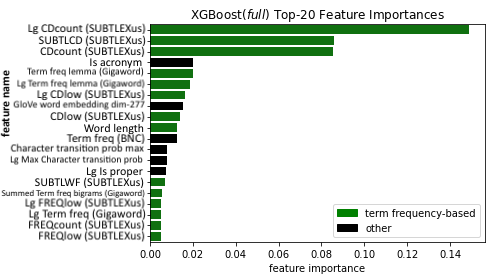
\includegraphics[scale=0.85]{xgboost_feature_importances.png}
  \captionsetup{justification=centering}
  \caption{\label{fig:xgboost_feature_importance} Feature importances for XGBoost(\textit{full}).}
\end{figure}

In total we consider 110 features, in addition to our multidimensional embedding-based features and $\log$-transformed features. We inspect the estimated feature importance scores produced by the XGBoost(\textit{full}) model to find that term frequency-based features (eg. unigrams, bigrams, trigrams) are of overwhelming importance (see Figure \ref{fig:xgboost_feature_importance}). This raises concern over whether the MT-DNN model too relies on term frequencies to make \textit{its} predictions, and if not, the linguistic features it may have learned upon fine-tuning. Of the remaining features having non-zero feature importances, most appear to be dimensions of a target word-based semantic feature (ie. GloVe or ELMo embeddings).

\section{BERT Attention}
\label{sec:bert_attention}

\begin{figure}
  \centering
  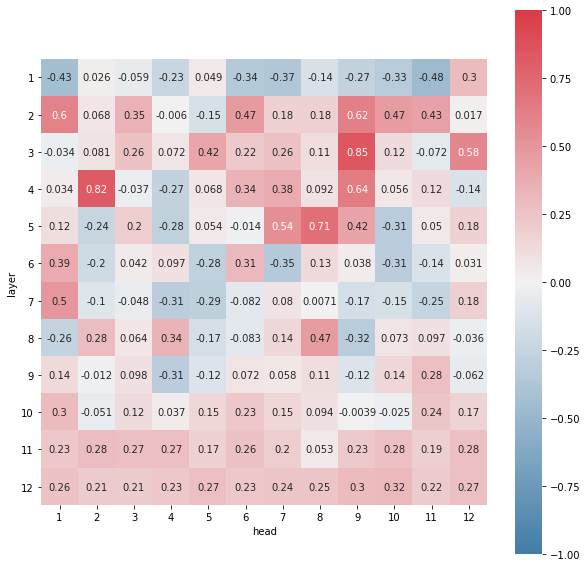
\includegraphics[scale=0.6]{head_correlations_tf.png}
  \captionsetup{justification=centering}
  \caption{\label{fig:head_correlations_tf} Attention head correlation between word frequency and total attention received by word, averaged across 100 random test set samples.}
\end{figure}

\begin{figure}
  \centering
  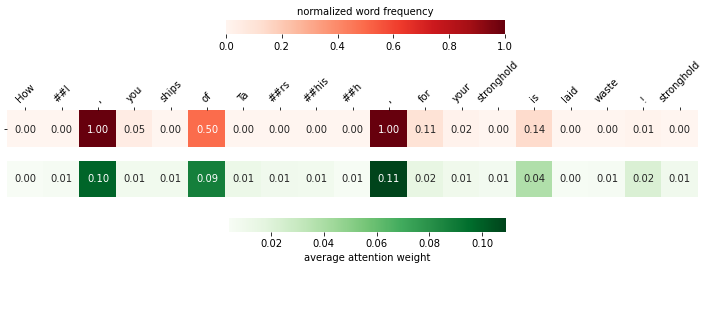
\includegraphics[scale=0.6]{head_3-9_tf_avg.png}
  \captionsetup{justification=centering}
  \caption{\label{fig:head_3-9_tf_avg} Word frequency vs. average head 3-9 attention weight directed to words of a random sample.}
\end{figure}

\begin{figure}
  \centering
  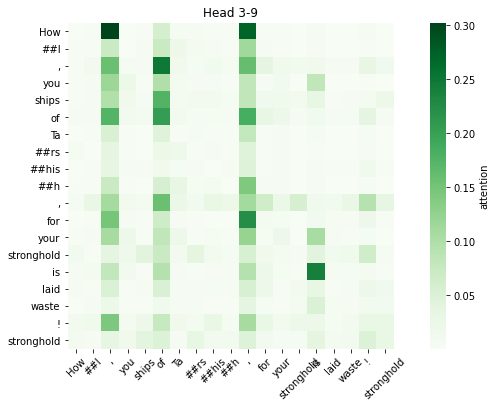
\includegraphics[scale=0.8]{head_3-9.png}
  \captionsetup{justification=centering}
  \caption{\label{fig:head_3-9} Head 3-9 attention map for a random sample.}
\end{figure}

\begin{figure}
  \centering
  
\includegraphics[scale=0.1]{images/pickle.png}
  \captionsetup{justification=centering}
  \caption{\label{fig:attn_feature_importances} This figure will show a heatmap of attention head importances measured using a gradient-based approach.}
\end{figure}

Attention maps of Transformers have in previous works been assessed to demonstrate linguistic phenomena learned by specialized attention heads \citep{190509418, 190604341}, and to measure the relative contribution of each attention head to making task predictions \citep{190509418, 190510650}. We extract attention maps from MT-DNN's underlying fine-tuned BERT architecture. For each sample in the single word test set, we obtain an attention map from each of the BERT base model's 144 attention heads (ie. 12 heads per 12 layers).

Based on the precedence given to term frequency features by the XGBoost(\textit{full}) model, we hypothesize that for certain attention heads, the degree to which BPEs attend to one another varies relative to the token's rarity in the lexicon. This follows the findings of \citealp{190509418}, who identify heads in which lesser frequent tokens are attended to semi-uniformly by a majority of sentence tokens. 

To test our hypothesis, we estimate for each attention head the Pearson correlation between word frequency and the average attention given to each word in the context.\footnote{We compute attention given to a \textit{word} as the sum of attention given to its constituent BPEs. We use the GBND corpus to extract word frequencies from, though any large corpora would suffice.} As illustrated in Figures \ref{fig:head_correlations_tf} and \ref{fig:head_3-9_tf_avg}, we find multiple attention heads appearing to specialize at directing attention towards the most or least frequent words (depending on sign of the correlation). Vertical stripe patterns like that in Figure \ref{fig:head_3-9} emerge as a result of attention originating from a spectrum of tokens. The findings seem to affirm the fundamental relevancy of word frequency to lexical complexity prediction, corroborating our intuitions.

This paragraph will discuss our interpretations of Figure \ref{fig:attn_feature_importances}.

\chapter{Conclusion}

In this paper, we report inspirations for systems submitted by \texttt{BigGreen} to LCP SharedTask 2021, achieving reasonable performance for the single word subtask by adapting ensemble methods upon feature engineering and feature learning-based models. We see potential in future deep learning approaches, acknowledging the need for strong word frequency-based handcrafted features for the time being. We surpass our submitted results for the MWE subtask by utilizing the predictive capabilities of our single word subtask models, under the assumption that MWE complexity is compositional with respect to its constituent tokens.

Avenues for improvement include better data aggregation, as the relative lack of class 4,5 samples hurts Pearson correlation across samples of especially extreme complexity. A future approach may involve synthetic data generation using SMOGN \citep{pmlrv74branco17a}. \citet{shardlow2020complex} acknowledge a reader's familiarity with a genre may affect his/her perceived complexity of a word, however the CompLex dataset lacks details on each annotator's expertise or background, which may offer valuable insights. Future studies may consider extracting multidimensional embeddings from the later layers of their deep learning models, potentially feeding these embeddings into feature engineering-based models.

\appendix

\chapter{Feature Descriptions}

Here, we describe in greater detail the various features that were experimented with for our feature engineering-based model. Note that while this discussion regards the single word subtask, for the MWE subtask we compute the same features but for each of the head and tail words, respectively.

\section{Lexical Features}

\begin{table}[H]
  \centering
  \begin{tabular}{>{\centering\arraybackslash}p{0.2\linewidth}>{\arraybackslash}p{0.7\linewidth}}
    \hline \textbf{Feature} & \textbf{Description} \\ \hline 
    \texttt{word\_len} & Character length of the target word.\\
    \hline 
    \texttt{num\_syllables} & Number of syllables in the target word, via the Syllables library.\\
    \hline 
    \texttt{is\_acronym} & Boolean for whether the target word is all capital letters.\\
    \hline 
  \end{tabular}
  \label{lexical_features}
\end{table}

\section{Semantic Features}

\begin{table}[H]
  \centering
  \begin{tabular}{>{\centering\arraybackslash}p{0.35\linewidth}>{\arraybackslash}p{0.6\linewidth}}
    \hline \textbf{Feature} & \textbf{Description} \\ \hline  
    \texttt{num\_hyperyms} & Number of hyperyms associated with the target word. The target word is initially disambiguated using NLTK's implementation of the Lesk algorithm for Word Sense Disambiguation (WSD) \citep{10.1145318723.318728}, which finds the WordNet Synset with the highest number of overlapping words between the context and different definitions of each Synset.\\
    \hline 
    \texttt{num\_hyponyms} & Number of hyponyms associated with the target word. Procedure for finding this is analogous to that for \texttt{num\_hyperyms}.\\
    \hline 
    \texttt{glove\_word} & 300-dimension embedding trained on Wikipedia-2014 and Gigaword for each target word. The target word is lowercased for simplicity.\\
    \hline 
    \texttt{elmo\_word} & 1024-dimension embedding train on the One Billion Word Benchmark corpus for each target word.\\
    \hline 
    \texttt{glove\_context} & 300-dimension average of GloVe word embeddings (see \texttt{glove\_word}) for each word in the given context. Each word is lowercased for simplicity.\\
    \hline 
    \texttt{infersent\_embeddings} & 4096-dimension InferSent embedding for the context.\\
    \hline 
  \end{tabular}
  \label{semantic_features}
\end{table}

\section{Phonetic Features}

\begin{table}[H]
  \centering
  \begin{tabular}{>{\centering\arraybackslash}p{0.4\linewidth}>{\arraybackslash}p{0.5\linewidth}}
    \hline \textbf{Feature} & \textbf{Description} \\ \hline
    \texttt{char\_transition\_min} & Minimum of the set of character transition probabilities for each character bigram in the target word. Ground truth character transition probabilities between any two English characters are estimated over the Gigaword corpus.\\
    \hline 
    \texttt{char\_transition\_max} & Maximum of the set described above.\\
    \hline 
    \texttt{char\_transition\_mean} & Mean of the set described above.\\
    \hline 
    \texttt{char\_transition\_std} & Standard deviation of the set described above.\\
    \hline 
    \texttt{phoneme\_transition\_min} & Minimum of the set of phoneme transition probabilities for each character bigram in the target word. Ground truth phoneme transition probabilities between any two phonemes are estimated over the Gigaword corpus. The phoneme set considered is that of the CMU Pronouncing Dictionary.\tablefootnote{\url{http://speech.cs.cmu.edu/cgi-bin/cmudict}}\\
    \hline 
    \texttt{phoneme\_transition\_max} & Maximum of the set described above.\\
    \hline 
    \texttt{phoneme\_transition\_mean} & Mean of the set described above.\\
    \hline 
    \texttt{phoneme\_transition\_std} & Standard deviation of the set described above.\\
    \hline
  \end{tabular}
  \label{phonetic_features}
\end{table}

\section{Word Frequency \& N-gram Features}

\subsection{Gigaword-based}

\begin{table}[H]
  \centering
  \begin{tabular}{>{\centering\arraybackslash}p{0.2\linewidth}>{\arraybackslash}p{0.7\linewidth}}
    \hline \textbf{Feature} & \textbf{Description} \\ \hline
    \texttt{tf} & Term frequency of the target word. Note that all term frequency-based features are computed using the Scikit-learn library's \texttt{CountVectorizer} \citep{scikitlearn}.\\
    \hline 
    \texttt{tf\_lemma} & Term frequency of the lemmatized target word. Lemmatization is performed using NLTK's WordNet Lemmatizer.\\
    \hline 
    \texttt{tf\_summed\_bpe} & Sum of the term frequencies of each BPE of the target word. BPE tokenization is performed using Hugging Face's BERT Tokenizer.\\
    \hline 
    \texttt{tf\_ngram\_2} & Sum of the term frequencies of each bigram in the context containing the target word.\\
    \hline 
    \texttt{tf\_ngram\_3} & Sum of the term frequencies of each trigram in the context containing the target word in the context.\\
    \hline 
    \texttt{tfidf} & Term frequency-inverse document frequency.\\
    \hline 
    \texttt{tfidf\_ngram\_2} & Sum of the term frequency-inverse document frequencies of each bigram in the context containing the target word.\\
    \hline 
    \texttt{tfidf\_ngram\_3} & Sum of the term frequency-inverse document frequencies of each trigram in the context containing the target word.\\
    \hline
  \end{tabular}
  \label{word_frequency_and_n_gram_features_gigaword_based}
\end{table}

\subsection{Google Ngram-based}

\begin{table}[H]
  \centering
  \begin{tabular}{>{\centering\arraybackslash}p{0.3\linewidth}>{\arraybackslash}p{0.6\linewidth}}
    \hline \textbf{Feature} & \textbf{Description} \\ \hline 
    \texttt{google\_ngram\_1} & Term frequency of the target word.\\
    \hline 
    \texttt{google\_ngram\_2\_head} & Term frequency of leading bigram in context containing the target word.\\
    \hline 
    \texttt{google\_ngram\_2\_tail} & Term frequency of trailing bigram in context containing the target word.\\
    \hline 
    \texttt{google\_ngram\_2\_min} & Minimum of the set of term frequencies of each bigram in context containing the target word.\\
    \hline 
    \texttt{google\_ngram\_2\_max} & Maximum of the set described above.\\
    \hline 
    \texttt{google\_ngram\_2\_mean} & Average of the set described above.\\
    \hline 
    \texttt{google\_ngram\_2\_std} & Standard deviation of the set described above.\\
    \hline 
    \texttt{google\_ngram\_3\_head} & Term frequency of leading trigram in context containing the target word.\\
    \hline 
    \texttt{google\_ngram\_3\_mid} & Term frequency of middle trigram in context containing the target word.\\
    \hline 
    \texttt{google\_ngram\_3\_tail} & Term frequency of trailing trigram in context containing the target word.\\
    \hline 
    \texttt{google\_ngram\_3\_min} & Minimum of the set of term frequencies of each trigram in context containing the target word.\\
    \hline 
    \texttt{google\_ngram\_3\_max} & Maximum of the set described above.\\
    \hline 
    \texttt{google\_ngram\_3\_mean} & Average of the set described above.\\
    \hline 
    \texttt{google\_ngrams\_3\_std} & Standard deviation of the set described above.\\
    \hline 
  \end{tabular}
  \label{word_frequency_and_n_gram_features_google_ngram_based}
\end{table}

\subsection{SUBTLEXus-based}

\begin{table}[H]
  \centering
  \begin{tabular}{>{\centering\arraybackslash}p{0.2\linewidth}>{\arraybackslash}p{0.7\linewidth}}
    \hline \textbf{Feature} & \textbf{Description} \\ \hline 
    \texttt{FREQcount} & Number of times the target word appears in corpus.\\
    \hline 
    \texttt{CDcount} & Number of films in which the target word appears.\\
    \hline 
    \texttt{FREQlow} & Number of times the lowercased target word appears in corpus.\\
    \hline 
    \texttt{CDlow} & Number of films in which the lowercased target word appears.\\
    \hline 
    \texttt{SUBTLWF} & Number of times the target word appears per million words.\\
    \hline 
    \texttt{SUBTLCD} & Percentage of films in which the target word appears.\\
    \hline 
  \end{tabular}
  \label{word_frequency_and_n_gram_features_SUBTLEXus_based}
\end{table}

\subsection{BNC-based}

\begin{table}[H]
  \centering
  \begin{tabular}{>{\centering\arraybackslash}p{0.3\linewidth}>{\arraybackslash}p{0.6\linewidth}}
    \hline \textbf{Feature} & \textbf{Description} \\ \hline 
    \texttt{bnc\_frequency} & Term frequency of the target word.\\
    \hline 
  \end{tabular}
  \label{word_frequency_and_n_gram_features_BNC_based}
\end{table}

\section{Syntactic Features}

\begin{table}[H]
  \centering
  \begin{tabular}{>{\centering\arraybackslash}p{0.45\linewidth}>{\arraybackslash}p{0.55\linewidth}}
    \hline \textbf{Feature} & \textbf{Description} \\ \hline 
    \texttt{parse\_tree\_depth} & Height of context's constituency parse tree. We get tree using Stanford CoreNLP pipeline.\\
    \hline 
    \texttt{token\_depth} & Depth of the target word with respect to root node of the context's constituency parse tree.\\
    \hline 
    \texttt{num\_words\_at\_depth} & Number of words at the depth of the target word in the context's constituency parse tree (see \texttt{token\_depth} above).\\
    \hline 
    \texttt{is\_proper} & Boolean for whether the target word is a proper noun/adjective, based on capitalization.\\
    \hline 
    \texttt{POS\_\{CC, CD, DT, EX, FW, IN, JJ, JJR, JJS, LS, MD, NN, NNP, NNPS, NNS, PDT, POS, PRP, PRP\$, RB, RBR, RBS, RP, SYM, TO, UH, VB, VBD, VBG, VBN, VBP, VBZ, WDT, WP, WP\$, WRB\}} & Booleans for whether the target word's part-of-speech tag is such. Tags considered are those used in the Penn Treebank Project.\tablefootnote{\url{https://www.ling.upenn.edu/courses/Fall_2003/ling001/penn_treebank_pos.html}} Tags are estimated using NLTK's \texttt{pos\_tag} method.\\
    \hline 
  \end{tabular}
  \label{syntactic_features}
\end{table}

\section{Readability Features}

\begin{table}[H]
  \centering
  \begin{tabular}{>{\centering\arraybackslash}p{0.5\linewidth}>{\arraybackslash}p{0.4\linewidth}}
    \hline \textbf{Feature} & \textbf{Description} \\ \hline 
    \texttt{automated\_readability\_index, avg\_character\_per\_word, avg\_letter\_per\_word, avg\_syllables\_per\_word, char\_count, coleman\_liau\_index, crawford, fernandez\_huerta, flesch\_kincaid\_grade, flesch\_reading\_ease, gutierrez\_polini, letter\_count, lexicon\_count, linsear\_write\_formula, lix, polysyllabcount, reading\_time, rix, syllable\_count, szigriszt\_pazos, SMOGIndex, DaleChallIndex} & Algorithms applied using the Textstat library's implementations, most of whom are readability metrics.\\
    \hline 
  \end{tabular}
  \label{readability_features}
\end{table}

\section{Other Features}

\begin{table}[H]
  \centering
  \begin{tabular}{>{\centering\arraybackslash}p{0.3\linewidth}>{\arraybackslash}p{0.6\linewidth}}
    \hline \textbf{Feature} & \textbf{Description} \\ \hline 
    \texttt{ppl} & Perplexity metric, as defined by the Hugging Face library.\tablefootnote{\url{https://huggingface.co/transformers/perplexity.html}} A pretrained GPT-2 model is used to obtain a log-likelihood for each token in the context, given its preceding tokens. A sliding-window approach is used to handle the large number of tokens in a context. The log-likelihoods are averaged, and finally exponentiated.\\
    \hline 
    \texttt{ppl\_aspect\_only} & Similar approach to that described above, where only log-likelihoods of tokens comprising the target word are averaged.\\
    \hline 
    \texttt{num\_OOV} & Number of words in the context that do not exist in the vocabulary of Gigaword.\\
    \hline 
    \texttt{corpus\_bible, corpus\_biomed, corpus\_europarl} & Booleans indicating the domain of the sample.\\
    \hline 
  \end{tabular}
  \label{other_features}
\end{table}

%%%%%%%%%%%%%%%%%%%%%%%%%%%%%%%%%%%%%%%%%%%%%%%%%%
%Backend of thesis (references and the like)
%%%%%%%%%%%%%%%%%%%%%%%%%%%%%%%%%%%%%%%%%%%%%%%%%%
\backmatter

%Add your bibliography filename and uncomment these lines
\addcontentsline{toc}{chapter}{References}
\bibliographystyle{acl_natbib}
\bibliography{anthology,acl2021}
\markboth{{\sffamily\sc Bibliography}}{}


%Uncomment if you want an index
%\printindex

\end{document}